\subsection{Objective Revision in a Mathematical Campaign}
\label{sec:vertical-trace}

Figure~\ref{fig:erdos-vertical-trace} follows the retained mathematical claim
frontier inside one real campaign. The case begins with an open-ended research objective.
The Manager preserves that goal through budget and process
failures; the Planner turns the current reviewed state into bounded work; the
Engineer retrieves sources, runs tools, and writes research artifacts; and the
Reviewer decides whether the work is accepted, revised, or blocked before it can
enter durable state.

\begin{figure}[H]
  \centering
  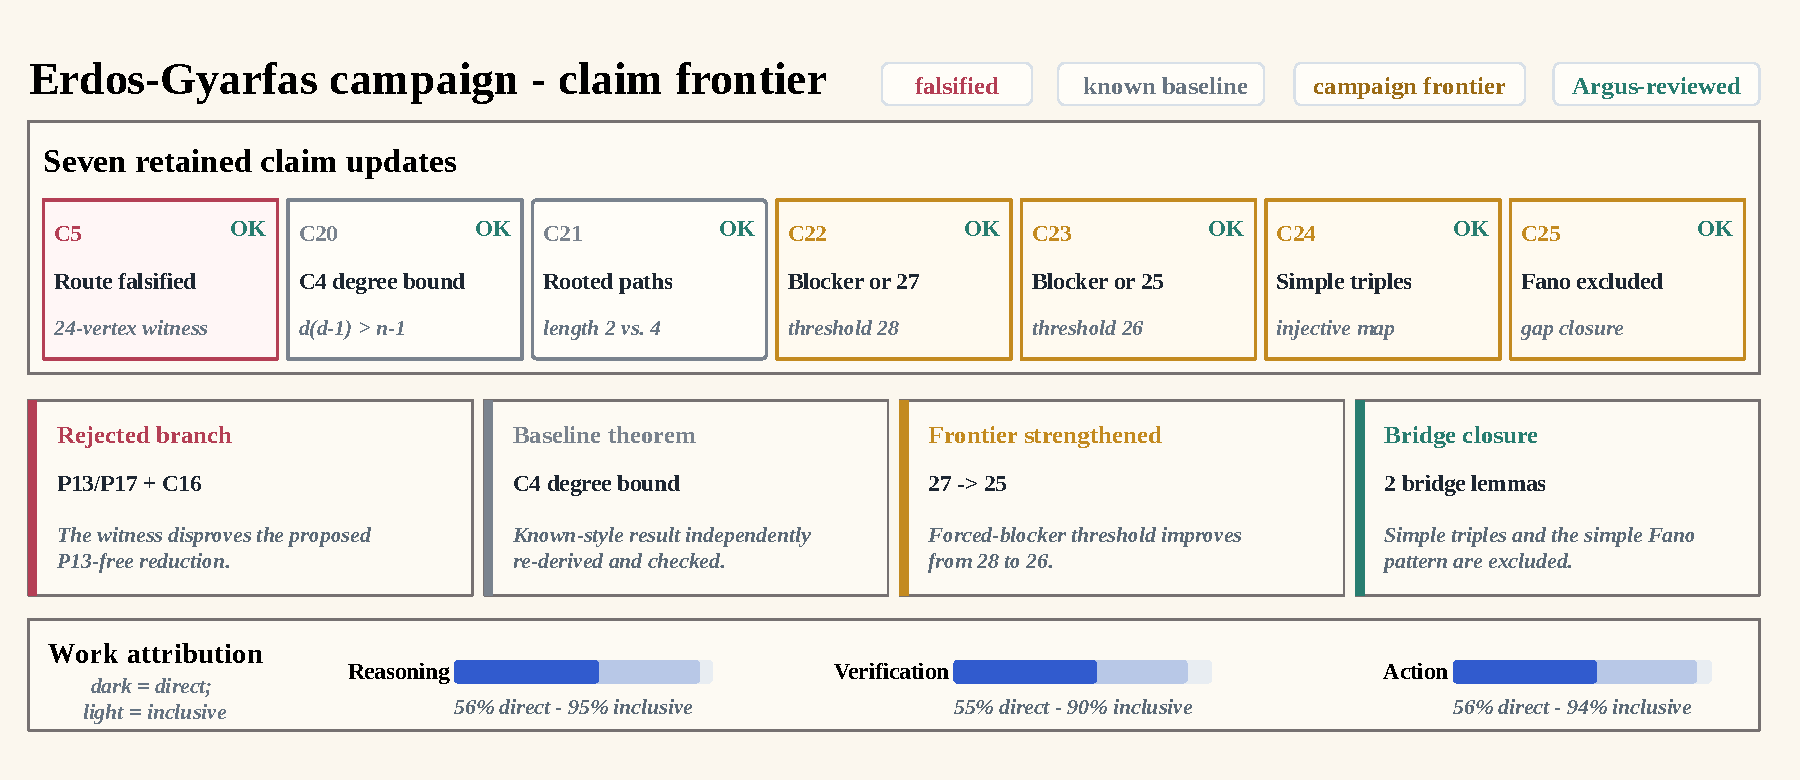
\includegraphics[width=\linewidth]{figures/erdos_vertical_trace.pdf}
  \caption{Reviewed claim frontier in the representative mathematical campaign.
  Seven retained updates progress from a falsified route (C5), through two
  independently re-derived baselines (C20--C21), to four campaign-frontier results
  (C22--C25), including the 27-to-25 strengthening and two bridge lemmas. The
  middle cards expose the corresponding artifacts, while the bottom bars separate
  direct frontier-changing work from an inclusive measure that also credits
  validation and state consolidation. Check marks indicate internal \systemname
  review, not external peer review or a novelty claim.}
  \label{fig:erdos-vertical-trace}
\end{figure}

The trace makes the work allocation concrete. The Manager recovers the campaign
and owns stage transitions. The Planner first selects a cheap falsification test,
then proposes changing the success contract from ``collect observations'' to
``produce a proof''; the Manager admits that refinement,
and later requires new missions to advance the retained result rather than restart
from an easier fact. The Engineer performs the domain work---source retrieval,
executable checks, proof writing, and result packaging. The Reviewer rejects an
overstated route, requests the missing checks, and certifies the bounded theorem
recorded by the artifacts.

In the reported trace, the campaign retains one falsified route and six proof-backed
deltas, including one stricter bound and two bridge results. Accepted work changes
the next Planner input, rejected work remains available as a dead branch, and open
blockers become explicit future tasks. The trace therefore captures a continuous
research path rather than a sequence of isolated answers.

\subsection{Efficiency Attribution in the Mathematical Case}

We apply Equation~\ref{eq:operational-efficiency} to the theorem-production
window covering Rounds 12--17. The analysis contains 18 bounded missions: six changed
the theorem frontier, four directly checked or re-certified mathematical results,
seven consolidated review state and documentation, and one overlap-analysis mission was interrupted
without an admitted result. Table~\ref{tab:erdos-efficiency} uses mission purpose as
a coarse attribution rule for process allocation.

\begin{table}[H]
\centering
\footnotesize
\renewcommand{\arraystretch}{1.12}
\begin{tabularx}{\linewidth}{@{}p{2.65cm}rrrX@{}}
\toprule
\rowcolor{papersand}
\textbf{Efficiency view} & \textbf{Direct} & \textbf{Auxiliary} & \textbf{Failed/no-op} & \textbf{Unit and interpretation} \\
\midrule
Reasoning & 56.0\% & 39.1\% & 4.9\% & Engineer reasoning-output Tokens; direct means a frontier-changing proof mission. \\
Verification & 55.4\% & 35.0\% & 9.6\% & Reviewer reasoning-output Tokens; direct means proof comparison or re-certification. \\
Action & 55.6\% & 38.9\% & 5.6\% & Mission count; direct comprises six frontier missions and four verification missions. \\
\bottomrule
\end{tabularx}
\caption{Efficiency attribution for the representative mathematical case.
Auxiliary work includes result packaging, checkpoint updates, and documentation
consolidation.}
\label{tab:erdos-efficiency}
\end{table}

The normalized interpretation is concrete. Of every 100 Engineer
reasoning-output Tokens, approximately 56 occurred in frontier-changing proof
missions, 39 in verification or state-maintenance work, and 5 in the interrupted
branch. Of every 100 Reviewer reasoning-output Tokens, approximately 55 directly
checked a proof package, 35 maintained formal review state, and 10 were
spent in the interrupted analysis. The strict action score is $10/18=55.6\%$; if the
seven successful auxiliary missions are also credited, the inclusive score is
$17/18=94.4\%$. Cost weighting makes the interruption more visible: the strict and
inclusive action scores become 56.1\% and 89.7\%, respectively.

The trace also clarifies what the numerator should reward. The early witness check
that killed a proposed reduction counts as an efficient action because it pruned a
false route before a long proof attempt. In Round 15, selecting one internal triple,
deriving the degree bounds, and closing the counting inequality are direct reasoning;
rewriting the result into the structured claim record is auxiliary work. Reviewer
inspection of those steps is direct verification, whereas updating the working
checkpoint is coordination overhead. This separation prevents activity volume from being mistaken for research
progress while preserving necessary coordination as a visible cost.
